% ---------------------------------------------------------------------------
%  GENERADO AUTOMATICAMENTE por scripts/07_deck_latex.py
%  Las cifras provienen de reports/metrics/*.json. Si reentrenas un modelo,
%  regenera este archivo en vez de editar los numeros a mano:
%      python scripts/07_deck_latex.py
%  (Igual puedes editarlo a mano: es LaTeX normal.)
% ---------------------------------------------------------------------------
\documentclass[aspectratio=169,11pt,table]{beamer}

\usepackage[utf8]{inputenc}
\usepackage[T1]{fontenc}
\usepackage{lmodern}
\usepackage[spanish,es-noshorthands]{babel}
\usepackage{graphicx}
\usepackage{booktabs}
\usepackage{array}
\usepackage{textcomp}
\usepackage{amssymb}

\graphicspath{{figuras/}}

% --- Paleta del proyecto ---------------------------------------------------
\definecolor{verdeosc}{HTML}{2E6B2F}
\definecolor{verdecla}{HTML}{8FB339}
\definecolor{grisTexto}{HTML}{444A52}
\definecolor{grisSuave}{HTML}{8A9098}
\definecolor{grisFondo}{HTML}{F6F7F4}
\definecolor{azul}{HTML}{1F6FB2}
\definecolor{rojo}{HTML}{D1495B}
\definecolor{morado}{HTML}{6A4C93}

% --- Tema ------------------------------------------------------------------
\usetheme{default}
\usefonttheme{professionalfonts}
\setbeamertemplate{navigation symbols}{}
\setbeamercolor{structure}{fg=verdeosc}
\setbeamercolor{normal text}{fg=grisTexto}
\setbeamercolor{frametitle}{fg=verdeosc}
\setbeamercolor{itemize item}{fg=verdecla}
\setbeamercolor{itemize subitem}{fg=verdecla}
\setbeamerfont{frametitle}{size=\Large,series=\bfseries}
\setbeamerfont{framesubtitle}{size=\scriptsize}
\setbeamertemplate{itemize item}{\raisebox{0.15ex}{\tiny$\blacksquare$}}
\setbeamertemplate{itemize subitem}{\raisebox{0.15ex}{\tiny$\square$}}

% Usa \par + \vspace en vez de \\ a proposito: con un subtitulo vacio, un \\
% despues de un grupo vacio provoca "There's no line here to end".
\setbeamertemplate{frametitle}{%
  \vspace*{0.35em}%
  \begin{beamercolorbox}[wd=\paperwidth,leftskip=0.7cm,rightskip=0.7cm]{frametitle}%
    \setlength{\parskip}{0pt}\setlength{\parindent}{0pt}%
    {\usebeamerfont{frametitle}\insertframetitle}\par
    {\usebeamerfont{framesubtitle}\color{grisSuave}\insertframesubtitle}\par
    \vspace{0.2em}%
    {\color{verdecla}\rule{1.7em}{2pt}}%
  \end{beamercolorbox}%
}

\setbeamertemplate{footline}{%
  \hfill{\tiny\color{grisSuave}\insertframenumber\,/\,\inserttotalframenumber}%
  \hspace{0.7cm}\vspace{0.25cm}%
}

% --- Atajos ----------------------------------------------------------------
% Linea de cierre al pie de un slide: el "take-away".
\newcommand{\cierre}[1]{%
  \vfill
  {\color{verdecla}\rule{2.5pt}{0.9em}}\hspace{0.4em}%
  {\footnotesize\color{grisSuave}#1}%
}
% Tarjeta tipo KPI: un numero grande con etiqueta.
\newcommand{\kpi}[4][verdeosc]{%
  \begin{minipage}[t]{#2}%
    \setlength{\fboxsep}{6pt}%
    \colorbox{grisFondo}{\begin{minipage}[t]{\dimexpr\linewidth-2\fboxsep-2\fboxrule\relax}%
      {\tiny\color{grisSuave}\bfseries #3}\\[0.12em]%
      % \large y no \Large: con cinco tarjetas en una fila, un valor como
      % "99,2 %" en \Large desborda la caja.
      {\large\bfseries\color{#1}#4}%
    \end{minipage}}%
  \end{minipage}%
}
% Caja con titulo y borde de color: para contraponer dos ideas lado a lado.
% Se dibuja con LaTeX, no como imagen: una figura hecha de texto queda
% ilegible en cuanto hay que reducirla para que entre en el slide.
\newcommand{\caja}[4][verdeosc]{%
  \begin{minipage}[t]{#2}%
    \setlength{\fboxsep}{7pt}%
    \fcolorbox{#1}{grisFondo}{\begin{minipage}[t]{\dimexpr\linewidth-2\fboxsep-2\fboxrule\relax}%
      {\small\bfseries\color{#1}#3}\\[0.45em]%
      #4%
      \vspace{0.2em}%
    \end{minipage}}%
  \end{minipage}%
}
\newcommand{\sig}{\textcolor{verdeosc}{\textbf{significativa}}}
\newcommand{\nosig}{\textcolor{rojo}{\textbf{NO significativa}}}

\renewcommand{\arraystretch}{1.25}
\setlength{\tabcolsep}{5pt}

% Descomenta para imprimir con notas del orador:
% \setbeameroption{show notes}

\title{Clasificación de madurez de paltas Hass --- Avance}
\author{Cristóbal Martínez, Benjamín Espinoza, Felipe Alvarez, Felipe Torres, Felipe Rojo}

\begin{document}

{
\setbeamercolor{background canvas}{bg=verdeosc}
\begin{frame}[plain]
  \vspace{1.4cm}
  % linespread: a \Huge el interlineado por defecto deja los descendentes de una
  % linea tocando la siguiente.
  {\color{white}\Huge\bfseries\linespread{1.15}\selectfont Clasificación del estado de\\madurez de paltas Hass}

  \vspace{0.55cm}
  {\color{verdecla}\rule{\textwidth}{1.6pt}}

  \vspace{0.55cm}
  {\color{white!85!verdecla}\large ResNet-50 frente a ViT-S/16 con presupuesto equiparado}

  \vfill
  % autor y fecha en lineas separadas: con varios autores la linea envuelve y
  % el separador queda colgando al borde derecho.
  {\color{white!70!verdecla}\small Cristóbal Martínez, Benjamín Espinoza, Felipe Alvarez, Felipe Torres, Felipe Rojo}

  \vspace{0.15em}
  {\color{white!70!verdecla}\small Avance, 21 de septiembre de 2026}

  \vspace{0.2em}
  {\color{white!60!verdecla}\footnotesize 14.710 fotografías, 478 frutas, índice de madurez de 5 niveles}
  \vspace{0.6cm}
\end{frame}
}

\begin{frame}{El problema}
\begin{columns}[T]
\begin{column}{0.58\textwidth}
{\scriptsize
\setlength{\itemsep}{0.3em}
\begin{itemize}
  \item {\bfseries Chile es uno de los mayores exportadores de palta Hass del mundo.}
  \item La clasificación por madurez se hace hoy a ojo y al tacto, operario por operario, sin criterio homogéneo ni trazabilidad.
  \item Fruta verde en góndola: el consumidor la descarta. Fruta pasada en tránsito: pérdida total. Los dos errores cuestan.
  \item {\bfseries La tarea es \emph{ordinal}, no categórica: $1<2<3<4<5$.}
  \item Confundir un 1 con un 2 es un error de un día. Confundir un 1 con un 5 es mandar fruta podrida a la venta.
\end{itemize}
}
\end{column}
\begin{column}{0.38\textwidth}
{\tiny
\centering
\begin{tabular}{cll}
\toprule
\rowcolor{verdeosc}\color{white}\bfseries Índ. & \color{white}\bfseries Estado & \color{white}\bfseries Decisión \\
\midrule
1 & Verde & Dejar madurar \\
2 & Iniciando & Lista en 2--3 días \\
3 & Maduro I & Venta inmediata \\
4 & Maduro II & Último día \\
5 & Sobremaduro & Fuera de punto \\
\bottomrule
\end{tabular}
}
\end{column}
\end{columns}
\cierre{La métrica tiene que castigar más los errores lejanos. La accuracy plana no lo hace: por eso usamos QWK.}
\end{frame}

\begin{frame}{Los datos}{Hass Avocado Ripening Photographic Dataset, Mendeley, CC BY 4.0}
\kpi[verdeosc]{0.224\textwidth}{Imágenes}{14.710}\hfill
\kpi[azul]{0.224\textwidth}{Frutas}{478}\hfill
\kpi[morado]{0.224\textwidth}{Clases}{5}\hfill
\kpi[rojo]{0.224\textwidth}{Grupos}{3}
\vspace{0.4em}
\begin{center}
  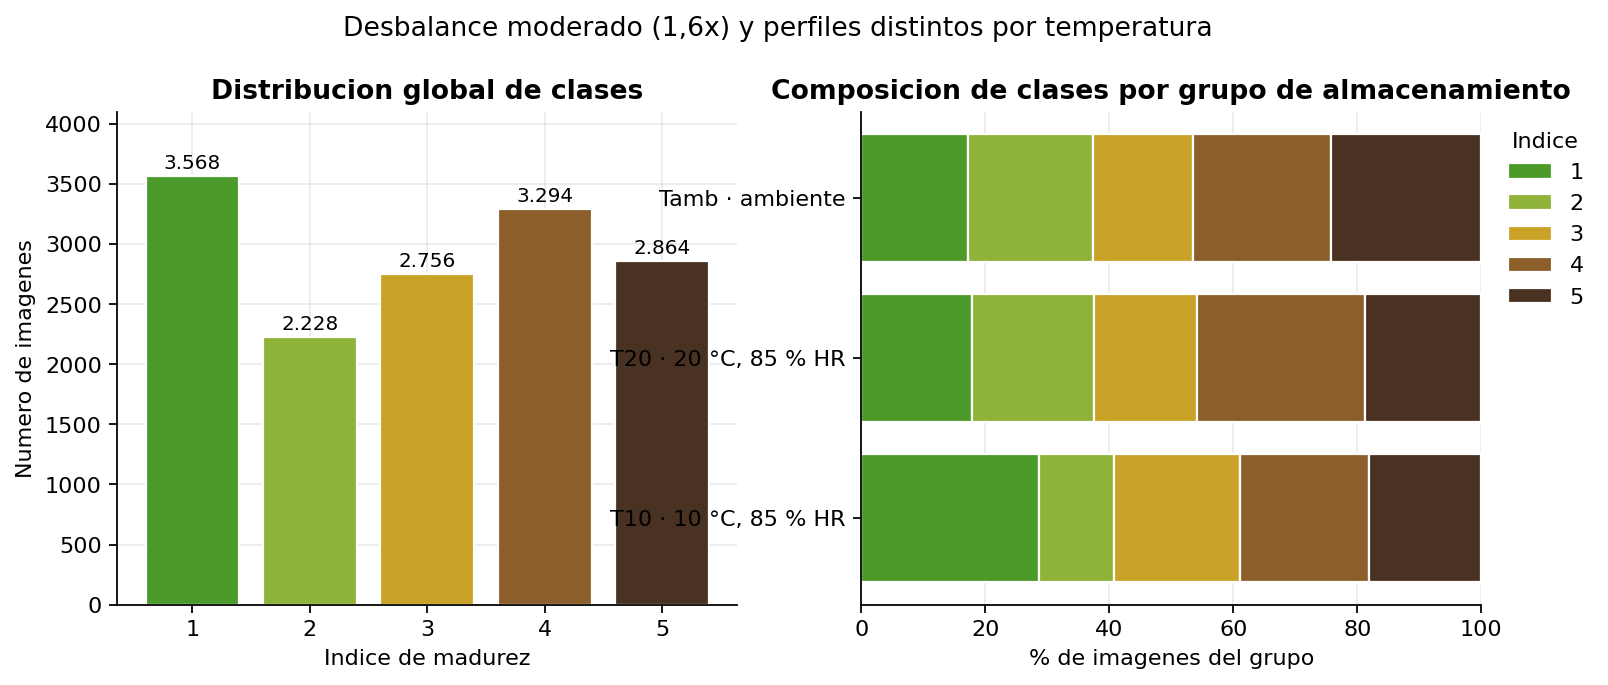
\includegraphics[width=0.84\textwidth,height=3.2cm,keepaspectratio]{01-distribucion-clases}
\end{center}
\cierre{Xavier, Rodrigues \& Silva (2024), DOI 10.17632/3xd9n945v8.1. Etiquetado visual experto, sin acuerdo inter-evaluador reportado.}
\end{frame}

\begin{frame}{El riesgo de que la IA haga trampa}
\begin{columns}[T]
\begin{column}{0.52\textwidth}
{\tiny
\setlength{\itemsep}{0.2em}
\begin{itemize}
  \item {\bfseries A cada palta le sacaron una foto por día, hasta 26 días seguidos.}
  \item La foto del día 5 y la del día 6 de la misma palta son casi idénticas: misma piel, mismas manchas, misma forma.
  \item {\bfseries Si repartimos las fotos al azar, la trampa es inevitable.}
  \item El día 5 queda en el material de estudio y el día 6 en la prueba. El modelo \emph{reconoce esa palta} en vez de juzgar su madurez, como un alumno que vio las respuestas antes del examen.
  \item El resultado saldría altísimo y sería completamente falso.
  \item {\bfseries Por eso repartimos las 478 paltas, no las 14.710 fotos.}
  \item Todas las fotos de una misma palta van juntas: o están en el estudio, o están en la prueba. Nunca en las dos.
\end{itemize}
}
\end{column}
\begin{column}{0.44\textwidth}
\begin{center}
  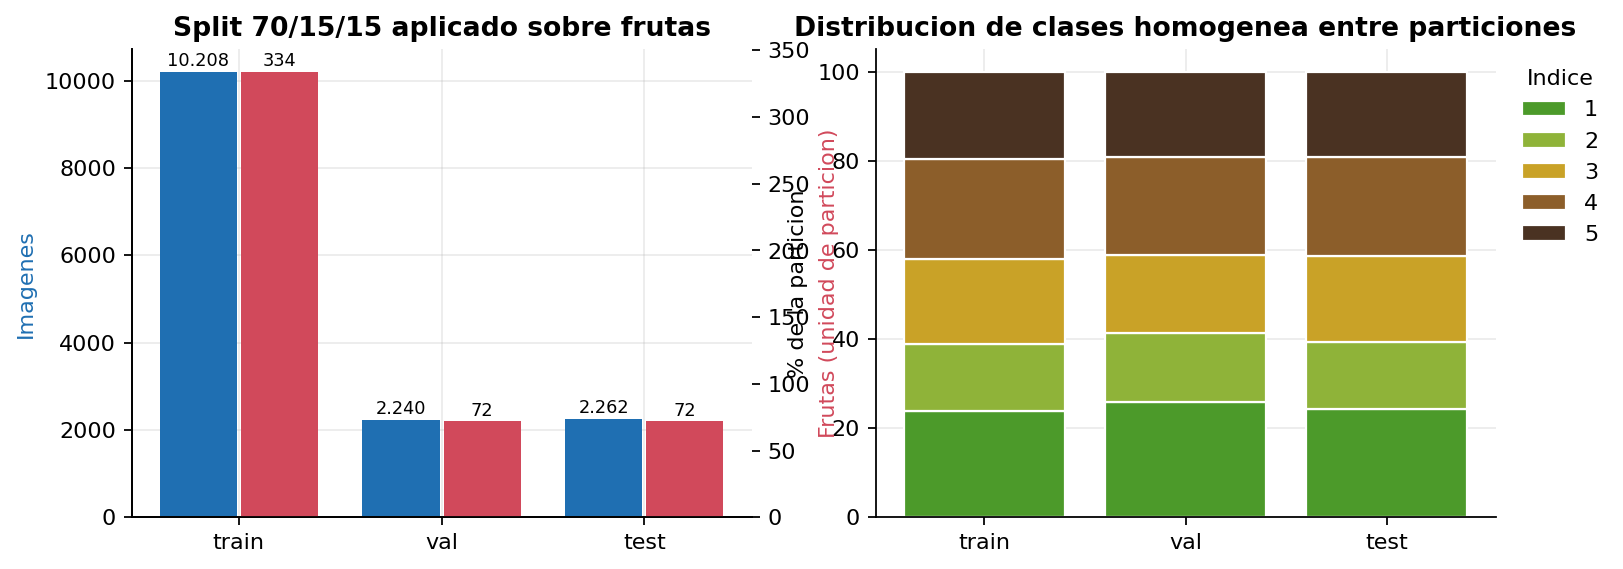
\includegraphics[width=\textwidth,height=2.9cm,keepaspectratio]{04-particiones}
\end{center}
\end{column}
\end{columns}
\cierre{Implementamos un chequeo automático que falla si alguna palta llegara a aparecer en los dos lados.}
\end{frame}

\begin{frame}{Las dos redes, en una imagen}{La diferencia es CÓMO miran la foto}
\begin{center}
  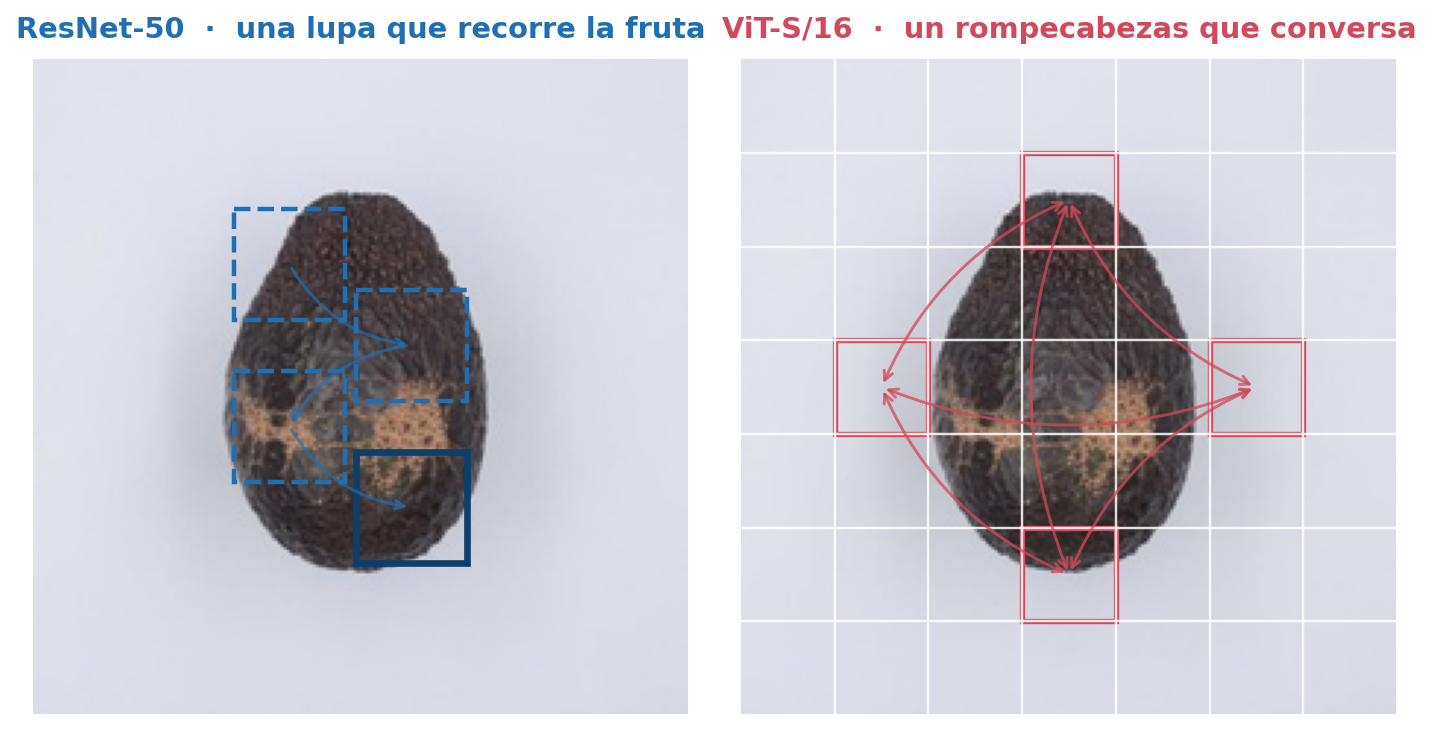
\includegraphics[width=0.95\textwidth,height=4.25cm,keepaspectratio]{30-como-mira-cada-red}
\end{center}
\vspace{0.25em}
\begin{columns}[T]
\begin{column}{0.47\textwidth}
{\tiny
\setlength{\itemsep}{0.12em}
\begin{itemize}
  \item Va de a pedacitos y reutiliza el mismo detector en toda la foto \textit{(convolución)}.
  \item Buena para detalles: manchas, arrugas, tono.
\end{itemize}
}
\end{column}
\begin{column}{0.47\textwidth}
{\tiny
\setlength{\itemsep}{0.12em}
\begin{itemize}
  \item Parte la foto en 196 cuadraditos y los compara todos contra todos \textit{(auto-atención)}.
  \item Buena para relacionar zonas distantes.
\end{itemize}
}
\end{column}
\end{columns}
\cierre{Ninguna se programó desde cero: las dos vienen de \texttt{timm}, la biblioteca estándar de modelos de visión.}
\end{frame}

\begin{frame}{Por qué entrenan tan distinto}{Todo se explica por lo que cada red ya sabe antes de empezar}
\caja[azul]{0.465\textwidth}{ResNet-50 trae dos reglas de fábrica}{{\scriptsize
\setlength{\itemsep}{0.1em}
\begin{itemize}
  \item Lo que importa está \textbf{cerca}
  \item \textbf{No importa} en qué parte de la foto esté
\end{itemize}
}
\vspace{0.25em}
{\tiny\color{grisSuave}\itshape Una mancha café es una mancha café, arriba o abajo de la fruta. Eso no lo aprende: ya lo trae.}}\hfill
\caja[rojo]{0.465\textwidth}{ViT-S/16 no trae ninguna}{{\scriptsize
\setlength{\itemsep}{0.1em}
\begin{itemize}
  \item Todos los cuadraditos le parecen \textbf{iguales}
  \item Ni siquiera sabe cuáles son \textbf{vecinos}
\end{itemize}
}
\vspace{0.25em}
{\tiny\color{grisSuave}\itshape Tiene que deducir de los ejemplos hasta la noción de \guillemotleft{}al lado\guillemotright{}.}}
\vspace{0.55em}
{\scriptsize
\setlength{\itemsep}{0.25em}
\begin{itemize}
  \item {\bfseries El ViT necesita muchísimos más ejemplos.}
  \item La ResNet arranca sabiendo mirar imágenes; el ViT tiene que descubrir primero \emph{cómo} se mira una imagen, y recién después aprender de paltas.
  \item {\bfseries Por eso los dos parten desde ImageNet.}
  \item Antes de ver una sola palta ya vieron 1,3 millones de fotos de cosas cotidianas. Ahí el ViT compensa su desventaja y llega con el oficio aprendido.
\end{itemize}
}
\end{frame}

\begin{frame}{Cómo hacemos que la comparación sea justa}{Igualar tres cosas, no solo el tamaño}
{\scriptsize
\centering
\begin{tabular}{lccc}
\toprule
\rowcolor{verdeosc}\color{white}\bfseries Qué igualamos & \color{white}\bfseries ResNet-50 & \color{white}\bfseries ViT-S/16 & \color{white}\bfseries Diferencia \\
\midrule
Tamaño del \guillemotleft{}cerebro\guillemotright{} (conexiones) & 23{,}5 millones & 21{,}7 millones & 7{,}9\,\% \\
Esfuerzo que hace por foto & 8{,}2 mil millones & 8{,}5 mil millones & 3{,}6\,\% \\
Fotos que vio antes de empezar & 1,3 millones & 1,3 millones & ninguna \\
\bottomrule
\end{tabular}
}
\vspace{0.5em}
{\scriptsize
\setlength{\itemsep}{0.25em}
\begin{itemize}
  \item {\bfseries Si una red es más grande y gana, no aprendimos nada: ganó por grande.}
  \item Por eso igualamos el tamaño (parámetros), el trabajo que hace por foto (GFLOPs) y cuántas fotos vio antes.
  \item El ViT que usa todo el mundo viene entrenado con 14 millones de fotos; la ResNet, con 1,3 millones. Comparándolos así estaríamos midiendo quién estudió más, no qué arquitectura es mejor.
  \item Usamos una versión del ViT llamada \textbf{DeiT-S}: es exactamente la misma red, pero entrenada con las mismas 1,3 millones de fotos que la ResNet. Ahí sí la comparación es limpia.
\end{itemize}
}
\end{frame}

\begin{frame}{Cómo las entrenamos}
\begin{columns}[T]
\begin{column}{0.47\textwidth}
{\small\textbf{Idéntico para ambas}}
{\scriptsize
\setlength{\itemsep}{0.16em}
\begin{itemize}
  \item Las mismas fotos, en el mismo orden
  \item Las mismas deformaciones de las fotos
  \item La misma cantidad de vueltas al dataset
  \item El mismo criterio para elegir el mejor modelo
  \item El mismo criterio para cortar el entrenamiento
\end{itemize}
}
\end{column}
\begin{column}{0.47\textwidth}
{\small\textbf{Distinto en el ViT}}
{\scriptsize
\setlength{\itemsep}{0.16em}
\begin{itemize}
  \item {\bfseries Learning rate 3 veces más pequeño.}
  \item Es el tamaño del paso. Con pasos largos el ViT tropieza y deja de aprender.
  \item {\bfseries Y un arranque más lento (\emph{warmup}).}
  \item Las primeras vueltas van a media máquina, pero a la larga es lo mejor para el ViT.
\end{itemize}
}
\end{column}
\end{columns}
\vspace{0.4em}
{\scriptsize\textbf{Observación:} en casi cualquier otra tarea conviene alterar mucho los colores de las fotos de entrenamiento, para que el modelo no dependa del color. Acá el color \emph{es} la respuesta: si alteramos mucho el tono, una palta clase 2 se vuelve idéntica a una clase 4 pero con la etiqueta vieja. Le estaríamos enseñando mal. Por eso el color casi no se toca; girar y recortar la foto, en cambio, sí.}
\cierre{Igualar el learning rate \guillemotleft{}por justicia\guillemotright{} no sería más justo: sería solo peor para el ViT.}
\end{frame}

{
\setbeamercolor{background canvas}{bg=grisFondo}
\begin{frame}[plain]
  \vfill
  \hspace{0.6cm}{\color{verdecla}\fontsize{54}{58}\selectfont\bfseries 01}%
  \hspace{0.5cm}{\color{verdeosc}\Huge\bfseries Resultados preliminares}
  \vfill
\end{frame}
}

\begin{frame}{Resultado: ResNet-50}{Un cerebro de 23{,}5 millones de conexiones, 10 minutos de entrenamiento}
\kpi[azul]{0.47\textwidth}{Acierta, o se pasa por un solo escalón}{99{,}2\,\%}\hfill
\kpi[azul]{0.47\textwidth}{Cuando se equivoca, se equivoca por}{0{,}26 escalones}
\vspace{0.45em}
{\scriptsize\color{grisSuave}Acierta la clase exacta en el 74{,}6\,\% de las fotos \; \textbullet\; puntaje con castigo (QWK) 0{,}936 \; \textbullet\; Macro-F1 0{,}735}
\vspace{0.6em}
{\scriptsize
\setlength{\itemsep}{0.22em}
\begin{itemize}
  \item {\bfseries Casi nunca se equivoca por mucho.}
  \item En 99{,}2\,\% de las fotos dice la clase correcta o una vecina. Confundir una palta verde con una podrida no le pasó nunca.
  \item {\bfseries Se equivoca por menos de medio escalón.}
  \item 0{,}26 en una escala de 5 niveles: del orden de medio día de maduración.
  \item {\bfseries Anda igual de bien en las tres temperaturas de almacenamiento.}
\end{itemize}
}
\cierre{Medido sobre 2.262 fotos de 72 paltas que el modelo nunca había visto.}
\end{frame}

\begin{frame}{Resultado: ViT-S/16}{Un cerebro de 21{,}7 millones de conexiones, 5 minutos de entrenamiento}
\kpi[rojo]{0.47\textwidth}{Acierta, o se pasa por un solo escalón}{99{,}5\,\%}\hfill
\kpi[rojo]{0.47\textwidth}{Cuando se equivoca, se equivoca por}{0{,}28 escalones}
\vspace{0.45em}
{\scriptsize\color{grisSuave}Acierta la clase exacta en el 72{,}2\,\% de las fotos \; \textbullet\; puntaje con castigo (QWK) 0{,}931 \; \textbullet\; Macro-F1 0{,}711}
\vspace{0.6em}
{\scriptsize
\setlength{\itemsep}{0.22em}
\begin{itemize}
  \item {\bfseries Casi nunca se equivoca por mucho.}
  \item En 99{,}5\,\% de las fotos dice la clase correcta o una vecina. Confundir una palta verde con una podrida no le pasó nunca.
  \item {\bfseries Se equivoca por menos de medio escalón.}
  \item 0{,}28 en una escala de 5 niveles: del orden de medio día de maduración.
  \item {\bfseries Anda igual de bien en las tres temperaturas de almacenamiento.}
\end{itemize}
}
\cierre{Medido sobre 2.262 fotos de 72 paltas que el modelo nunca había visto.}
\end{frame}

\begin{frame}{ResNet-50 frente a ViT-S/16}{El resultado central del avance}
\begin{center}
  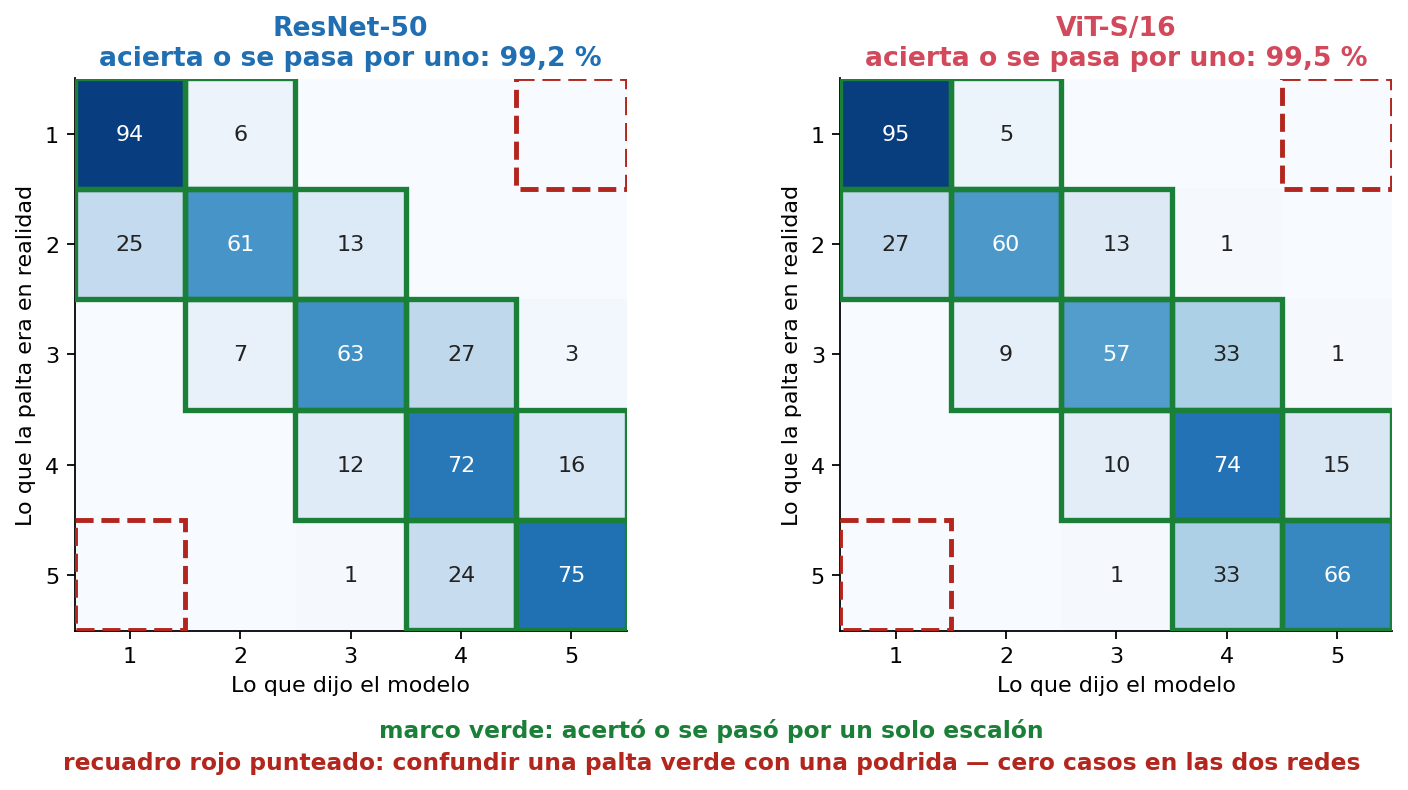
\includegraphics[width=0.86\textwidth,height=3.6cm,keepaspectratio]{33-matrices-didactica}
\end{center}
\vspace{0.3em}
{\tiny
\setlength{\itemsep}{0.2em}
\begin{itemize}
  \item {\bfseries Las dos rinden prácticamente igual.}
  \item La ResNet acierta la clase exacta un poco más seguido. Pero cuando el ViT se equivoca, se equivoca por menos. Se compensa.
  \item Hicimos la prueba estadística formal y la diferencia entre ambas no es concluyente: para efectos prácticos, empatan.
  \item {\bfseries Pero no se equivocan en las mismas fotos.}
  \item Fallan las dos a la vez en solo 18{,}0\,\% de los casos. Si alguien pudiera elegir siempre cuál de las dos tiene razón, acertaría 82{,}0\,\% en vez de 74{,}6\,\%.
  \item Eso es lo que van a intentar aprovechar los modelos híbridos.
\end{itemize}
}
\cierre{Los números completos y las pruebas estadísticas están en el anexo.}
\end{frame}

\begin{frame}{Curvas de entrenamiento}{Misma receta, convergencia distinta}
\begin{center}
  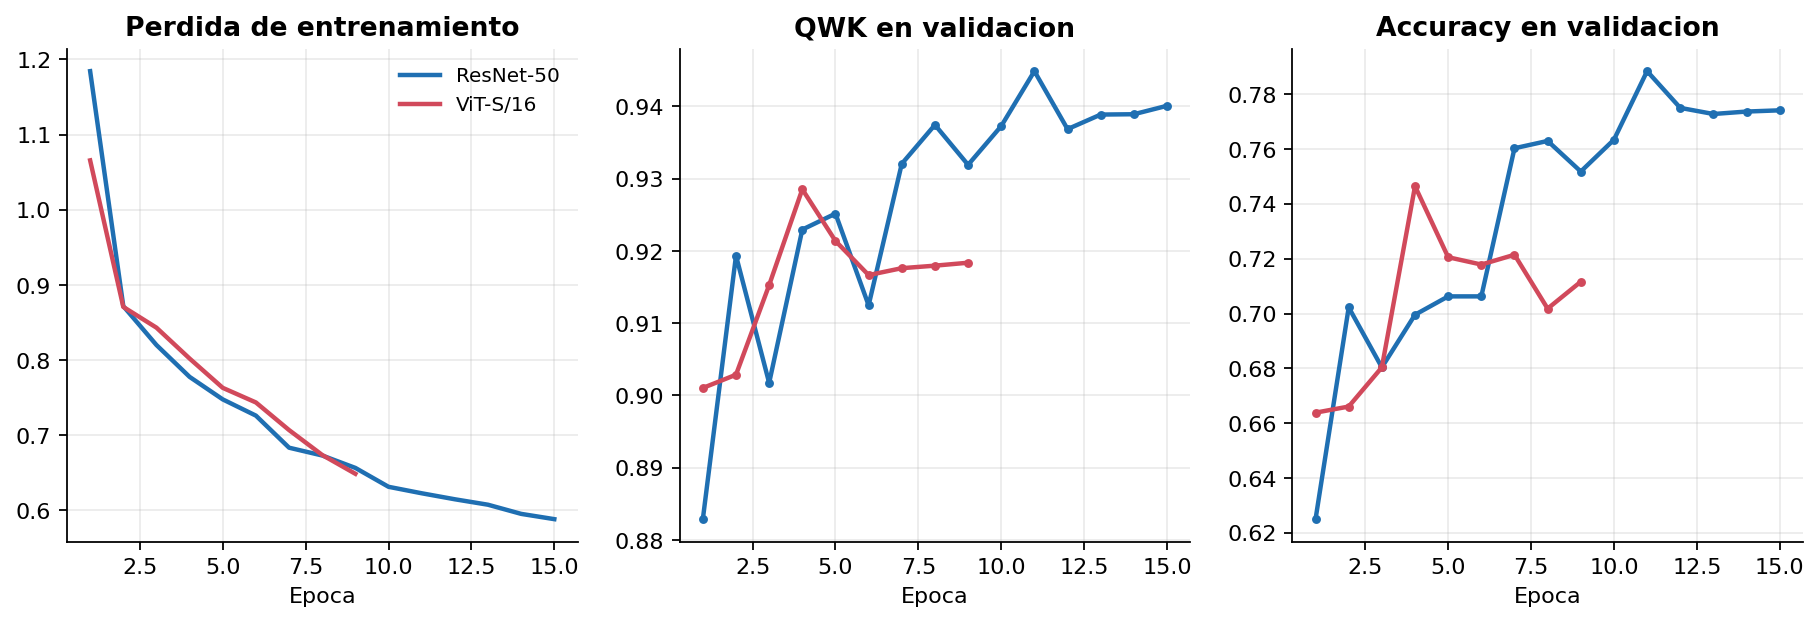
\includegraphics[width=\textwidth,height=4.3cm,keepaspectratio]{11-curvas-entrenamiento-avance}
\end{center}
\vspace{0.3em}
{\scriptsize
\setlength{\itemsep}{0.2em}
\begin{itemize}
  \item ResNet-50 alcanza su mejor QWK de validación en la época 11; ViT-S/16 en la 4.
  \item Tiempo de entrenamiento: 10 min frente a 5 min en una RTX 4070 Laptop de 8\,GB. El ViT converge al doble de velocidad.
\end{itemize}
}
\end{frame}

\begin{frame}{Riesgos identificados y mitigación}{Concretos de este dataset, no genéricos}
{\tiny
\centering
\begin{tabular}{>{\raggedright\arraybackslash}p{0.20\textwidth}>{\raggedright\arraybackslash}p{0.38\textwidth}>{\raggedright\arraybackslash}p{0.34\textwidth}}
\toprule
\rowcolor{verdeosc}\color{white}\bfseries Riesgo & \color{white}\bfseries Por qué es real acá & \color{white}\bfseries Qué hicimos \\
\midrule
Que la IA haga trampa & Hay 6.871 pares de fotos casi idénticas de la misma palta & Repartir paltas, no fotos, con chequeo automático \\
El choque con la vida real & Las fotos son de laboratorio: fondo blanco, luz perfecta, una fruta centrada. Un packing no se parece a eso & Lo declaramos como la limitación principal. Hay que salir a sacar fotos con celular \\
Alterar el color arruinaría el aprendizaje & El color \emph{es} la respuesta: si lo cambiamos, la etiqueta queda mal & Alteramos el color lo mínimo; giramos y recortamos sin problema \\
Una temperatura domina los datos & El grupo refrigerado aporta el 60\,\% de las fotos y casi todas las paltas verdes & Compensamos en el entrenamiento y revisamos el resultado temperatura por temperatura \\
Nadie sabe cuál es el techo & Las etiquetas las puso una persona mirando; no hay una segunda opinión con qué contrastar & Usamos métricas que perdonan el error de un escalón y no perseguimos el 100\,\% \\
Darle ventaja a una de las dos redes & El ViT que se usa por defecto vino entrenado con 14 millones de fotos, no 1,3 & Elegimos la versión del ViT que vio exactamente las mismas fotos que la ResNet \\
\bottomrule
\end{tabular}
}
\end{frame}

\begin{frame}{Qué viene para el entregable final}
{\scriptsize
\setlength{\itemsep}{0.25em}
\begin{itemize}
  \item {\bfseries Desarmar el modelo para ver qué pieza importa.}
  \item Reentrenar las dos redes sin ImageNet, solo con las fotos de paltas. Debería mostrar que el ViT depende mucho más de haber estudiado antes.
  \item {\bfseries Dos formas de juntar ambas redes en una.}
  \item Una que las hace opinar por separado y combina las dos respuestas; otra que las encadena, con la parte convolucional alimentando a la otra.
  \item {\bfseries Ver dónde mira cada red.}
  \item Pintar sobre la foto las zonas que cada modelo usó para decidir, sobre todo en los casos donde las dos discrepan.
  \item {\bfseries Una demo que funcione: subir una foto y ver la respuesta.}
  \item {\bfseries Y una recomendación explícita: cuál llevaríamos a una planta real, pesando precisión contra costo.}
\end{itemize}
}
\end{frame}

{
\setbeamercolor{background canvas}{bg=grisFondo}
\begin{frame}[plain]
  \vfill
  \hspace{0.6cm}{\color{verdecla}\fontsize{54}{58}\selectfont\bfseries A}%
  \hspace{0.5cm}{\color{verdeosc}\Huge\bfseries Anexo}
  \vfill
\end{frame}
}

\begin{frame}{Anexo: todas las métricas}{Test: 2.262 imágenes de 72 frutas nunca vistas}
{\scriptsize
\centering
\begin{tabular}{lcccccccc}
\toprule
\rowcolor{verdeosc}\color{white}\bfseries Modelo & \color{white}\bfseries Params & \color{white}\bfseries GFLOPs & \color{white}\bfseries QWK & \color{white}\bfseries Accuracy & \color{white}\bfseries Macro-F1 & \color{white}\bfseries MAE & \color{white}\bfseries Acc. $\pm$1 & \color{white}\bfseries min \\
\midrule
ResNet-50 & 23{,}5\,M & 8{,}2 & 0{,}9356 & 74{,}6\,\% & 0{,}735 & 0{,}262 & 99{,}2\,\% & 10 \\
ViT-S/16 & 21{,}7\,M & 8{,}5 & 0{,}9313 & 72{,}2\,\% & 0{,}711 & 0{,}282 & 99{,}5\,\% & 5 \\
\bottomrule
\end{tabular}
}
\vspace{0.5em}
{\tiny
\setlength{\itemsep}{0.18em}
\begin{itemize}
  \item \textbf{QWK}: kappa de Cohen con pesos cuadráticos. Penaliza el error según el cuadrado de la distancia entre clases y corrige por acuerdo azaroso. Es la métrica con la que elegimos el mejor modelo.
  \item \textbf{MAE}: error medio en escalones del índice de madurez.
  \item \textbf{Acc. $\pm$1}: fracción de predicciones en la clase correcta o una adyacente.
  \item \textbf{Macro-F1}: F1 promediado por clase; controla que las clases minoritarias no queden abandonadas.
\end{itemize}
}
\end{frame}

\begin{frame}{Anexo: pruebas estadísticas}{Diferencias contra ResNet-50, con intervalo de confianza del 95\,\%}
{\scriptsize
\setlength{\itemsep}{0.25em}
\begin{itemize}
  \item {\bfseries ViT-S/16: $\Delta$QWK $= $-$0{,}0042$, IC 95\,\% $[$-$0{,}0095, +0{,}0006]$, $p=0{,}095$ $\rightarrow$ \nosig}
  \item Los intervalos y los $p$-valores salen de un \emph{bootstrap pareado agrupado por fruta}: las 2.262 imágenes vienen de solo 72 paltas, así que remuestrear imágenes daría intervalos artificialmente angostos. Se remuestrean frutas, 2.000 réplicas.
\end{itemize}
}
\end{frame}

\begin{frame}{Anexo: desglose por temperatura de almacenamiento}{Sirve para detectar si el modelo se apoya en un atajo}
{\tiny
\centering
\begin{tabular}{llccc}
\toprule
\rowcolor{verdeosc}\color{white}\bfseries Modelo & \color{white}\bfseries Grupo & \color{white}\bfseries n & \color{white}\bfseries Accuracy & \color{white}\bfseries MAE \\
\midrule
ResNet-50 & T10 (10\,\textdegree C) & 1350 & 75{,}3\,\% & 0{,}259 \\
ResNet-50 & T20 (20\,\textdegree C) & 466 & 75{,}1\,\% & 0{,}249 \\
ResNet-50 & Tamb & 446 & 71{,}8\,\% & 0{,}285 \\
ViT-S/16 & T10 (10\,\textdegree C) & 1350 & 73{,}9\,\% & 0{,}267 \\
ViT-S/16 & T20 (20\,\textdegree C) & 466 & 68{,}7\,\% & 0{,}318 \\
ViT-S/16 & Tamb & 446 & 71{,}1\,\% & 0{,}291 \\
\bottomrule
\end{tabular}
}
\end{frame}

\end{document}
